% This is samplepaper.tex, a sample chapter demonstrating the
% LLNCS macro package for Springer Computer Science proceedings;
% Version 2.20 of 2017/10/04
%
\documentclass[runningheads]{llncs}
%
\usepackage{graphicx}
\usepackage{hyperref}
% Used for displaying a sample figure. If possible, figure files should
% be included in EPS format.
%
% If you use the hyperref package, please uncomment the following line
% to display URLs in blue roman font according to Springer's eBook style:
% \renewcommand\UrlFont{\color{blue}\rmfamily}

\begin{document}
%
\title{SPANG: constructing a controlled set of queries with the FAIR principle}
%
\titlerunning{SPANG library}
% If the paper title is too long for the running head, you can set
% an abbreviated paper title here
%
%\author{First Author\inst{1}\orcidID{0000-1111-2222-3333} \and
%Second Author\inst{2,3}\orcidID{1111-2222-3333-4444} \and
%Third Author\inst{3}\orcidID{2222--3333-4444-5555}}
\author{Hirokazu Chiba}
%
\authorrunning{H. Chiba}
% First names are abbreviated in the running head.
% If there are more than two authors, 'et al.' is used.
%
%\institute{Princeton University, Princeton NJ 08544, USA \and
%Springer Heidelberg, Tiergartenstr. 17, 69121 Heidelberg, Germany
%\email{lncs@springer.com}\\
%\url{http://www.springer.com/gp/computer-science/lncs} \and
%ABC Institute, Rupert-Karls-University Heidelberg, Heidelberg, Germany\\
%\email{\{abc,lncs\}@uni-heidelberg.de}}
\institute{Database Center for Life Science, Chiba 277-0871, Japan\\
\email{chiba@dbcls.rois.ac.jp}
}
%
\maketitle              % typeset the header of the contribution
%
\begin{abstract}
%The abstract should briefly summarize the contents of the paper in 15--250 words.
How can we maximize the value of accumulated SPARQL queries? An increasing number of datasets have been published in the Resource Description Framework (RDF) and the SPARQL standard allows interoperable framework for querying the RDF datasets; however, reuse of SPARQL queries remains in a limited level. The problem is the lack of findability, accessibility and reusability of SPARQL queries that were once written. 
%Given that SPARQL is an important framework of the Semantic Web, it is important to consolidate the eco-system to reuse SPARQL queries written in various project.
%Here, we present a extended specification for storing and distributing SPARQL queries named SPANG, and provide a pilot study of SPANG library.
Here we propose a SPARQL extention to construct a reusable query library to enrich the Semantic Web platform.
As a use case, we constructed a reusable SPARQL query library, named SPANG library.
Specifically, We challenged the issue of findability and accessibility of SPARQL queries.
This specification leads to the construction of eco-system to reuse SPARQL queries to enrich the use of the Semantic Web platform.
% These features facilitate easy access to RDF datasets by users. 
Our contributions are as follows.
1) We present a metadata set for annotating a SPARQL query.
It enables to identify SPARQL query, and provides useful information fo the query.
2) We also present a mechanism to parameterize the SPARQL query.
It make each query reusable in different settings.
Further, the mechanism enables federated queries by combining multiple queries through Unix pipe. 
% Here, we developed spang command, as a client that helps users to generate queries. SPANG can create typical short queries according to the arguments specified by users like a \textit{one-liner} style in the Unix command line. It can also call SPARQL template libraries constructed in a local file system or published on the Web. 
This study make SPARQL queries more findable, accessible, interoperable, and reusable, i.e., pushing forward FAIR SPARQL.
SPANG is freely available at \url{https://spang.dbcls.jp}.
\keywords{SPARQL query \and RDF store \and template library.}
\end{abstract}
%
%
%
\section{Introduction}
An increasing number of datasets have been published in the Resource Description Framework (RDF). 
Although the SPARQL language provides a basis for exploiting RDF databases, writing a raw SPARQL code often becomes a burden for users. 
% Several approaches for support of SPARQL writing exist. One is to develop SPARQL editors that have useful functionalities 
% such as URI autocompletion~\cite{Rietveld}.
% Another aims at automatic generation of SPARQL queries~\cite{Yamaguchi}.
% Despite the efforts of previous studies, Semantic Web users remain bound to the task of SPARQL coding.
Here, we developed SPANG, a novel SPARQL client
that addresses this issue of SPARQL coding by simple query generation and reusing existing query templates.
SPANG
%, with its unique features, 
minimizes the burden of coding SPARQL,
thereby enhancing integrative analysis of distributed RDF databases. 


SPARQL is a fundamental technology for querying RDF data. However, is is not designed for reusability. In data management guideline, FAIR principle is well known~\cite{fair}. Findability, Accesibility, Reusablility should be addressed, to make the most of SPARQL queries as resources. 

The Semantic Web is comprised of various specifications, including RDF~\cite{rdf}, OWL~\cite{owl}, and SPARQL~\cite{sparql}. The ontologies written in OWL are accumulated and shared on repositories~\cite{bioportal}.
RDF datasets are also accumulated and hosted in portal web sites~\cite{rdf-portal}.
Not only the ontologies and datasets, but also the queries are important for the Semantic Web.
Accumulating and reusing the queries are important.

Reusing SPARQL queries are important for efficient development of the Semantic Web. 

Are SPARQL queries accessible? In most cases, those queries are not accessible. According to the FAIR principle, resources should be accessible by through URI. In some cases, SPARQL queries are stored in repositories. But they do not have stable URIs.

How about findability? In many Semantic Web projects, SPARQL queries are written and accumulated. However, those SPARQL queries are not findable, due to the lack of export and import SPARQL queries.

Here, we decided to follow the FAIR principle and extend the SPARQL specifications for more efficient development of the Semantic Web.



The SPANG package includes the main {\tt spang} command, which can be used in the Unix command-line environment.
In general, the {\tt spang} command help users query RDF databases by dynamically generating SPARQL queries according to the command-line options or arguments. 
More specifically, {\tt spang} has two execution modes: 
1) simple mode; for a simple query, users must only specify some command-line options to generate the query without writing any SPARQL code, and
2) template mode; for a more complex query, users can generate the query using a predefined SPARQL template and parameters.
Basically, each {\tt spang} process submits a query to a specific database,
and the {\tt spang} process can be combined with other Unix processes through a Unix pipe. 
Notably, multiple {\tt spang} commands each with distinct target database can be combined through a Unix pipe, thereby realizing federated queries to multiple databases (see Section 2.4). 

To reduce the burden of coding SPARQL, the SPANG package provides predefined configurations about nicknames for SPARQL endpoints, prefix declarations for URIs, and SPARQL libraries (see Section 3).


Contributions of this work:
we provide a SPARQL meta data required for constucting SPARQL queries.
we constructed template engines for SPARQL queries.
we constructed controlled SPARQL queries for available SPARQL endpoints.


The following section includes: overview of the SPANG project, specification of SPANG templates, implementation of the SPANG library, and use case of SPANSG library.

%%%%%%%%%%%%%%%%%%%%%%%%
\section{The FAIR principle}

Not only the RDF dataset, but also the SPARQL queries are important resource to be shared on the Semantic Web platform. Thus, we applied the FAIR principle which have been applied to the RDF datasets, into SPARQL queries.

Here we overview the preliminaries for the FAIR principle.
It shoulbe noted that the FIAR principle can be applied not only to the dataset resources but also to other type of resources including software tools.

Here, we provide the FAIR principle in the context of SPARQL queries.

\subsection{Findable}
\begin{itemize}
    \item Assign global identifier
    \item Rich metadata
    \item Include the identifier of the data they describe
    \item Registered and indexed
\end{itemize}

\subsection{Accessible}
\begin{itemize}
    \item Retrievable by identifier
    \item Metadata are accessible
\end{itemize}

\subsection{Interoperable}
\begin{itemize}
    \item Use a formal, accessible, shared, and broadly applicable language for knowledge representation.
    \item Use vocabularies that follow FAIR principles.
    \item Include qualified references to others
\end{itemize}

\subsection{Reusable}
\begin{itemize}
    \item Richly described with a plurality of accurate and relevant attributes
    \begin{itemize}
        \item released with a clear and accessible data usage license
        \item associated with detailed provenance
        \item meet domain-relevant community standards
    \end{itemize}
\end{itemize}


%%%%%%%%%%%%%%%%%%%%%%%%
\section{SPANG overview}
Here we overview the structure of this paper.

\subsection{SPARQL metadata}

We propose a set of SPARQL metadata to annotate each SPARQL query, to make them more reusable.
Those metadata are added as comment at the head of the SPARQL query, thus that does not violate the SPARQL specification. 
The set of metadata increase the findability of SPARQL queries.

As a use case, we developed a SPANG API to search for the set of SPARQL queries.

\subsection{SPARQL parameterization}

We propose the parapeterization mechanism of SPARQL query. It is crucial to reuse the SPARQL query for us to improve the productivity of the programming experiance on the Semantic Web platform.

Using SPANG API, users can execute SPARQL query over the Web, with the given parameters.

\subsection{SPANG library}

According to the metadata and parameterization mechanism, we can construct a controlled set of SPARQL library which is reusable in various settings.

\subsection{SPANG command}

As an interface the the SPANG library, we constructed a command-line interface.

\subsection{SPANG portal}
SPANG is originally developed for "SARQLing" the RDF dataset from command line. Here, we re-implemented the SPANG using Node.js and now the functionality is available through Web browser. 

Figure~\ref{fig:spang_top} is the top page of SPANG, which includes links to GitHub, Documentation, and SPANG library.

\begin{figure}
\center
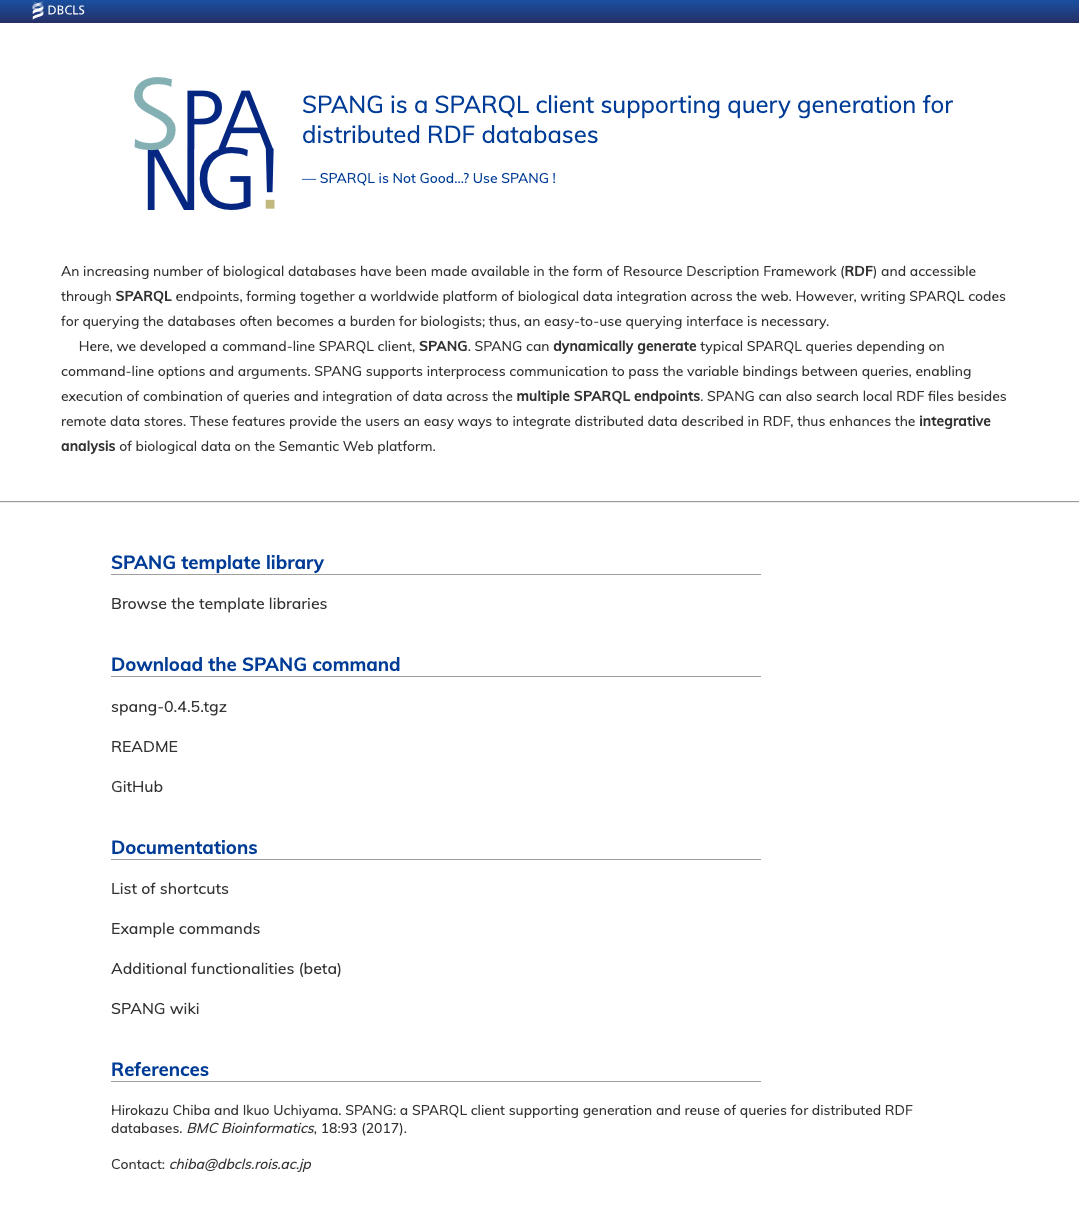
\includegraphics[width=1.0\textwidth]{spang_top.png}
\caption{SPANG web site}
\label{fig:spang_top}
\end{figure}

Figure~\ref{fig:spang_lib} is the list of the target SPARQL endpoints. It also lists the SPARQL templates available in general for various endpoints.

\begin{figure}
\center
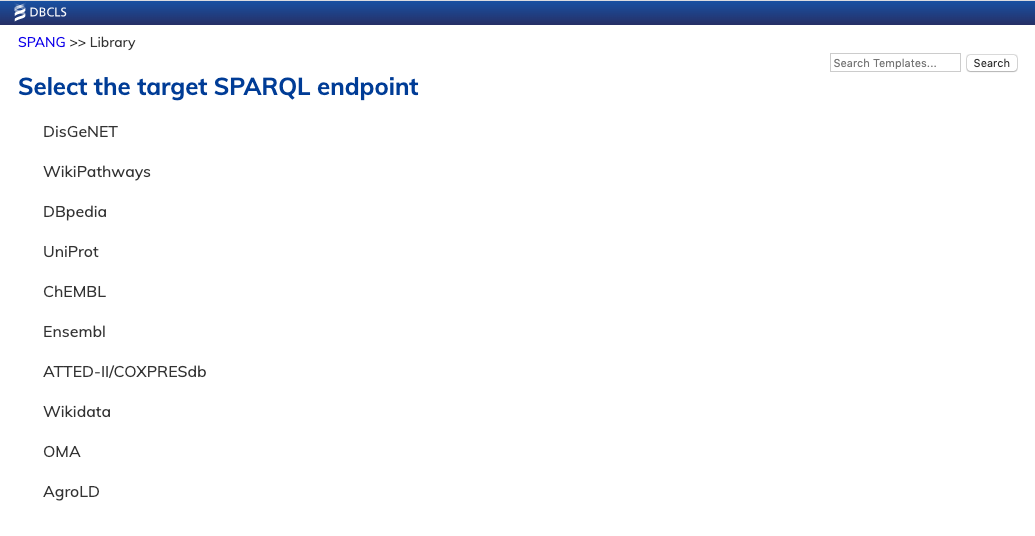
\includegraphics[width=1.0\textwidth]{spang_lib.png}
\caption{SPANG library}
\label{fig:spang_lib}
\end{figure}

Figure~\ref{fig:spang_lib} is the list of SPARQL templates for DisGeNet SPARQL endpoint.
A short name for the SPARQL template, descriptin of the query, and example parameters are shown.

\begin{figure}
\center
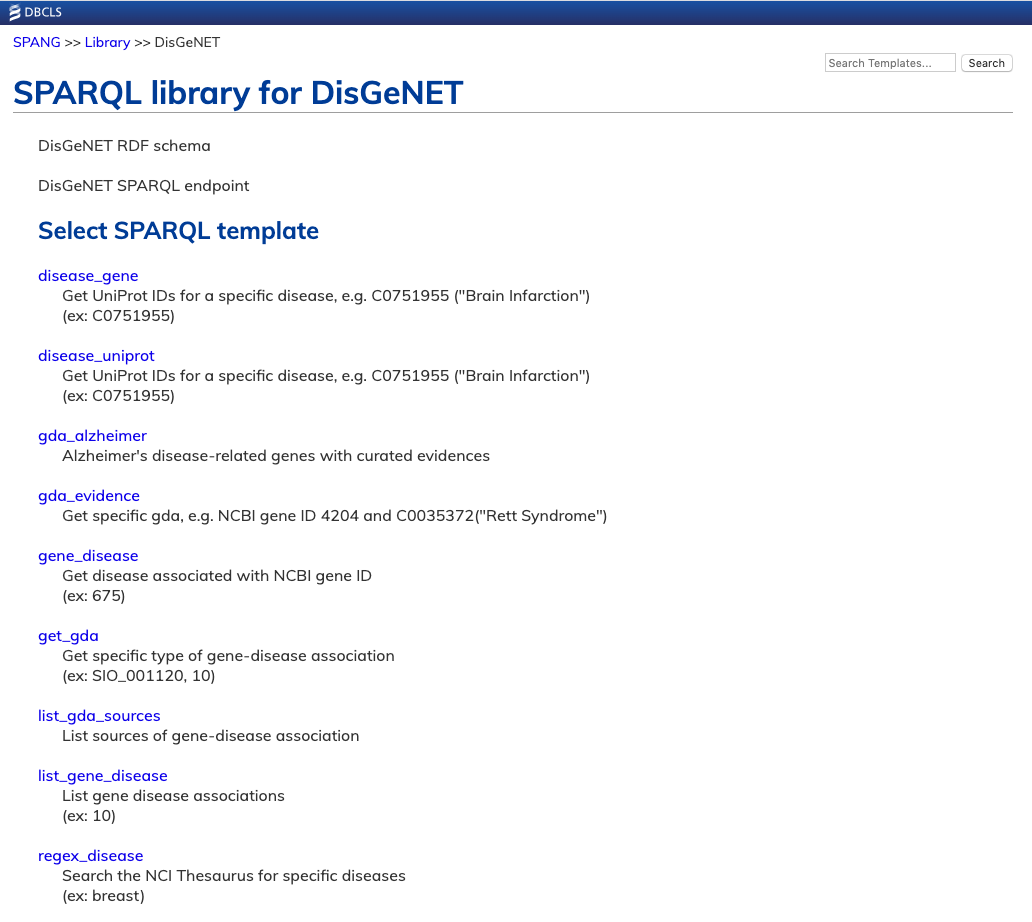
\includegraphics[width=1.0\textwidth]{spang_disgenet.png}
\caption{SPANG templates for DisGeNet SPARQL endpoint}
\label{fig:spang_disgenet}
\end{figure}

Figure~\ref{fig:spang_disease_gene_query} shows a query for DiesGeNet SPARQL endpoint to get disase gene relationship. 
Figure~\ref{fig:spang_disease_gene_result} shows the result of the query. Thus, users can get the results only by clicking on the web pages, browsing the SPARQL template on the SPANG web site.

\begin{figure}
\center
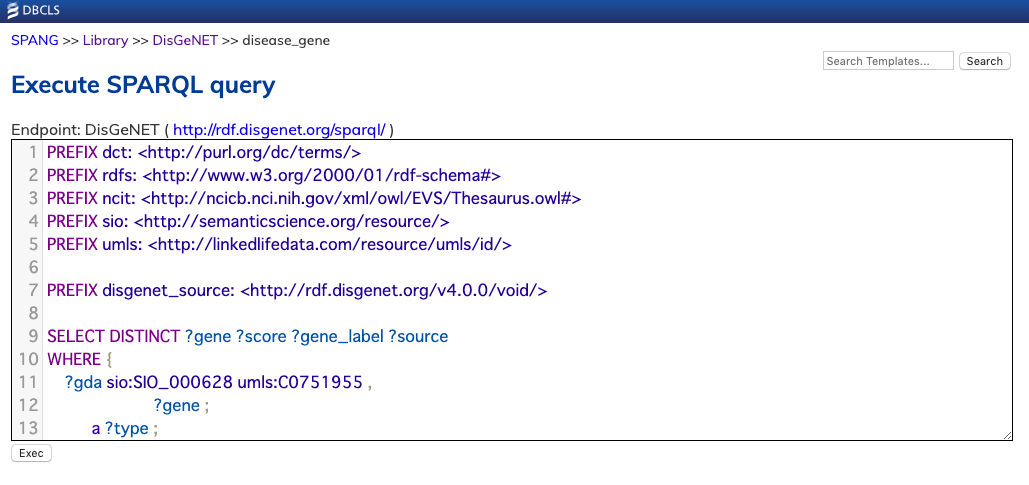
\includegraphics[width=1.0\textwidth]{spang_disease_gene_query.png}
\caption{SPANG templates for DisGeNet SPARQL endpoint}
\label{fig:spang_disease_gene_query}
\end{figure}

\begin{figure}
\center
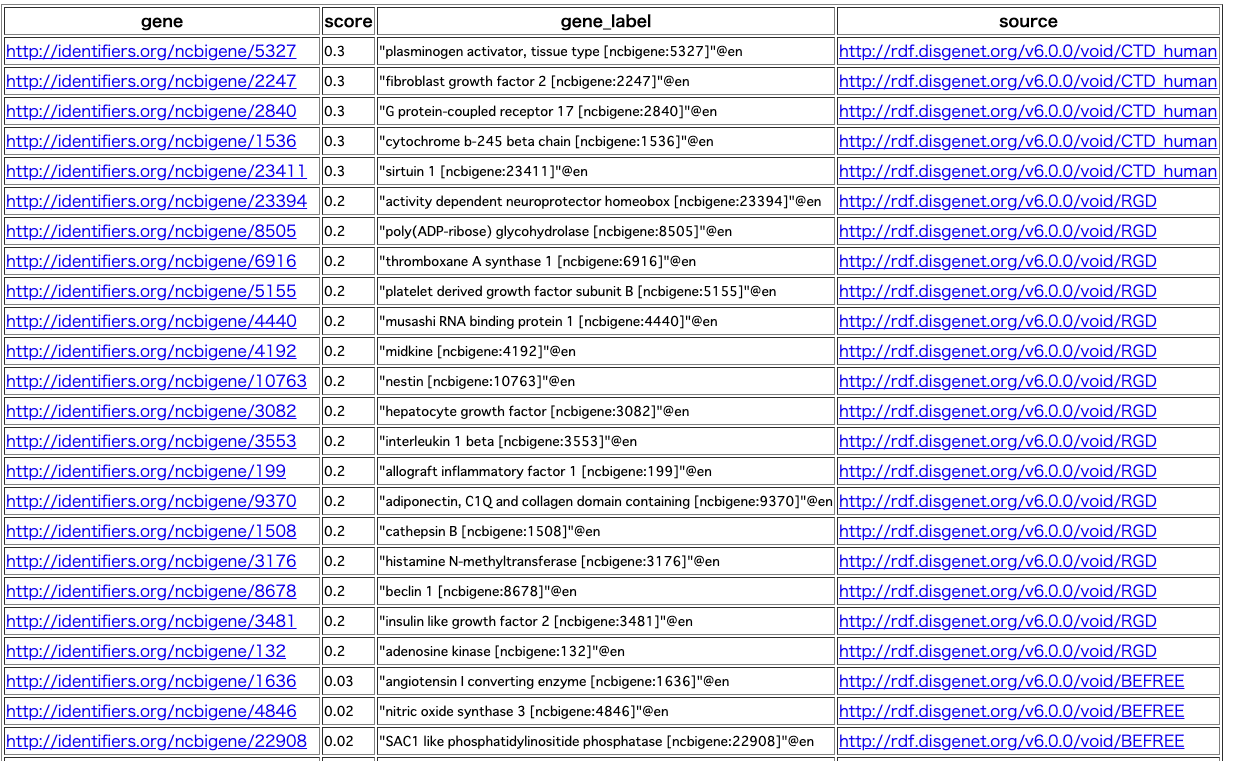
\includegraphics[width=1.0\textwidth]{spang_disease_gene_result.png}
\caption{SPANG templates for DisGeNet SPARQL endpoint}
\label{fig:spang_disease_gene_result}
\end{figure}


%%%%%%%%%%%%%%%%%%%%%%%%
\section{SPANG specifications}

Here, we constructed SPANG library: a SPARQL library which is findable, accessible, interoperable and reusable.

\subsection{Findability of SPARQL queries}
Most of the SPARQL queries are not findable from general users of the Semantic Web. The first and most important step toward increased value of the written SPARQL queries is to consider how to make SPARQL queries findable.
In the FAIR principle, making resources findable includes indexing resources by adding metadata to each resources. 
To make SPARQL queries findable, we propose to add metadata to SPARQL.
The SPARQL metadata includes:
\begin{itemize}
    \item Title
    \item Description
    \item Topic
    \item Parameters: name, default value, class
    \item Target endpoint
\end{itemize}

Indexing of SPARQL queries are conducted and thus users can obtain specific queries of interest through a search API.

\subsection{Accessibility to SPARQL queries}
Some of the SPARQL libraries are accessible from internet. Howver, we could consider more general scheme for accesibility. In the FAIR principle, accessibility includes minting URI for each resource. Here we propose to use stable URI for each SPARQL query.
In the case of SPANG library, we assign two URI for each query. One is for retrieving SPARQL query string, thereby users can retrieve the concrete content of the query. Another is URI to get results. This URI can include the parameter settings for the specified query.

\subsection{Interoperability of SPARQL}
SPARQL specification is proposed for interoperable use of queries to the Semantic Web. It is valuable to use several triplestore implementation through the same programming interface. However, no rule is proposed for coding rules; capitalization, indentation and newline, etc. Lack of those rules result in variation of SPARQL queries, which hampers the reuse of SPARQL queries. In other languages, some coding ruels exist. In the case of SPARQL, specification document or text books do not follow a specific coding rules. Here, we specify the coding rule used in SPANG template library, and implemented spfmt command to reformat of the code.

\subsubsection{SPANG coding rules}
We defined a coding rule for SPARQL and its extention in SPANG framework. Coding rule is important for productivity of shared coding tasks and effective maintenance. It also helps to make debug process easier; weird look suggests possible bugs. 
\begin{itemize}
    \item Header lines: query can start with header lines as comment lines. Metadata can be added at the top of the query as comment lines. Multiple lines are allowed. If multiple lines are described, they are written in sequential without blank lines. After the metadata lines, a blank line comes.
    \item Prefix: prefix declaration comes in sequential lines. Each of before and after the prefix declaration lines, a blank line exists.
    \item Cases: the SPARQL keywords should be in upper case characters. variabl names comes with ? followed by lower case characters.
    \item Literal: the literals are surrounded by "".
    \item Indent: indentation depth is two spaces.
    \item Spaces: a space exists between keywords and variables. A space exists before , or ; or . .
    \item Newline: a newline exists before the keyword \texttt{WHERE} and after \texttt{\{}. A new line exist after ; or . but not after ,. After the newline following ;, an indent follows. A newline exist before query modifiers such as \texttt{ORDER BY} or \texttt{LIMIT}.
\end{itemize}
We developed a reformatter of the SPARQL code as described below.

\subsection{Reusability of SPARQL queries}
Reusability of SPARQL is not a new topic. Various activity is conducted to construct libraries of SPARQL. It is considered as acitivities to increase the reusability of SPARQL queries. However, no standard to increase the reusability is proposed. In the specifiation of SPARQL, reusability is not a centroal topic. However, it is an central resource in a Semantic Web. If it is a component of Semantic Web comprised of RDF/OWL/SPARQL, it is reasonable to represent it in RDF framework. We propose a way to represent SPARQL in the RDF framework.

Templating is also a key issue for reusability. SPARQL specifications do not includes templating mechanism, but without templating, each SPARQL queries are not applicable to other use cases. We implemented templating mechanism using a general freamework, mustash.




\subsection{Example query}
An example query in the SPANG library is shown below.
The DisGeNet endpoint is specified.

\begin{figure}[!t]
\begin{scriptsize}
\begin{verbatim}
# @title Get UniProt IDs for a specific disease, e.g. C0751955 ("Brain Infarction")
# @endpoint http://rdf.disgenet.org/sparql/
# @prefix https://raw.githubusercontent.com/hchiba1/spang-library/master/prefix/bio
# @param arg1=C0751955 

PREFIX disgenet_source: <http://rdf.disgenet.org/v4.0.0/void/>
PREFIX umls: <http://linkedlifedata.com/resource/umls/id/>

SELECT DISTINCT ?gene ?score ?gene_label ?source ?gda ?pmid ?description
WHERE {
    ?gda sio:SIO_000628 umls:{{arg1}} ,
                        ?gene ;
          a ?type ;
          sio:SIO_000253 ?source ;
          sio:SIO_000216/sio:SIO_000300 ?score .
    ?gene a ncit:C16612 ;
          rdfs:label ?gene_label .
    OPTIONAL {
        ?gda sio:SIO_000772 ?pmid ;
             dct:description ?description .
    }
}
ORDER BY DESC(?score) ?source ?pmid

\end{verbatim}
\end{scriptsize}
\caption{Example query in SPANG library}
\label{fig:example-rdf}
\end{figure}

%%%%%%%%%%%%%%%%%%%%%%%%%
\section{SPANG API}

SPANG library is accesible through SPANG Web API.

\subsection{Library API}

\subsection{Query API}

The following command returns the list of query libraries.

\texttt{curl https://spang-portal.dbcls.jp/api/library}

\begin{figure}[!t]
\begin{scriptsize}
\begin{verbatim}
[
  {
    "name": "disgenet",
    "title": "DisGeNET",
    "description": "DisGeNET",
    "endpoint": "http://rdf.disgenet.org/sparql/",
    "schema": "http://www.disgenet.org/web/DisGeNET/menu/rdf#schema",
    "uri": "http://localhost:7070/api/library/disgenet",
    "count": 14
  },
  {
    "name": "wikipathways",
    "title": "WikiPathways",
    "description": "WikiPathways",
    "endpoint": "http://sparql.wikipathways.org/",
    "schema": null,
    "uri": "http://localhost:7070/api/library/wikipathways",
    "count": 6
  },
  ...
]
\end{verbatim}
\end{scriptsize}
\caption{List of in query libraries obtained by API}
\label{fig:example-rdf}
\end{figure}

The following command returns the result of the query, with the given paramter.

\texttt{curl https://spang-portal.dbcls.jp/api/library/disgenet/gene\_disease.rq?arg1=678}

\begin{figure}[!t]
\begin{scriptsize}
\begin{verbatim}

"Precursor T-Cell Lymphoblastic Leukemia-Lymphoma"@en	"0.31"^^<http://www.w3.org/2001/XMLSchema#double>	<http://identifiers.org/pubmed/28671688>	"2017"^^<http://www.w3.org/2001/XMLSchema#gYear>
"Precursor T-Cell Lymphoblastic Leukemia-Lymphoma"@en	"0.31"^^<http://www.w3.org/2001/XMLSchema#double>	<http://identifiers.org/pubmed/20622884>	"2010"^^<http://www.w3.org/2001/XMLSchema#gYear>
"Colorectal Cancer"@en	"0.3"^^<http://www.w3.org/2001/XMLSchema#double>	<http://identifiers.org/pubmed/25944804>	"2016"^^<http://www.w3.org/2001/XMLSchema#gYear>
"Colorectal Carcinoma"@en	"0.3"^^<http://www.w3.org/2001/XMLSchema#double>	<http://identifiers.org/pubmed/25944804>	"2016"^^<http://www.w3.org/2001/XMLSchema#gYear>
"Colorectal Neoplasms"@en	"0.3"^^<http://www.w3.org/2001/XMLSchema#double>	<http://identifiers.org/pubmed/25944804>	"2016"^^<http://www.w3.org/2001/XMLSchema#gYear>
"Malignant neoplasm of prostate"@en	"0.3"^^<http://www.w3.org/2001/XMLSchema#double>	<http://identifiers.org/pubmed/17199135>	"2007"^^<http://www.w3.org/2001/XMLSchema#gYear>
"Prostatic Neoplasms"@en	"0.3"^^<http://www.w3.org/2001/XMLSchema#double>	<http://identifiers.org/pubmed/17199135>	"2007"^^<http://www.w3.org/2001/XMLSchema#gYear>
"Lymphocyte Count measurement"@en	"0.1"^^<http://www.w3.org/2001/XMLSchema#double>	<http://identifiers.org/pubmed/27863252>	"2017"^^<http://www.w3.org/2001/XMLSchema#gYear>
"Platelet Count measurement"@en	"0.1"^^<http://www.w3.org/2001/XMLSchema#double>	<http://identifiers.org/pubmed/27863252>	"2017"^^<http://www.w3.org/2001/XMLSchema#gYear>
"Acute leukemia"@en	"0.01"^^<http://www.w3.org/2001/XMLSchema#double>	<http://identifiers.org/pubmed/21109922>	"2011"^^<http://www.w3.org/2001/XMLSchema#gYear>
"Burkitt Lymphoma"@en	"0.01"^^<http://www.w3.org/2001/XMLSchema#double>	<http://identifiers.org/pubmed/21109922>	"2011"^^<http://www.w3.org/2001/XMLSchema#gYear>
"Hematologic Neoplasms"@en	"0.01"^^<http://www.w3.org/2001/XMLSchema#double>	<http://identifiers.org/pubmed/21109922>	"2011"^^<http://www.w3.org/2001/XMLSchema#gYear>
"Leukemia, Myelocytic, Acute"@en	"0.01"^^<http://www.w3.org/2001/XMLSchema#double>	<http://identifiers.org/pubmed/21109922>	"2011"^^<http://www.w3.org/2001/XMLSchema#gYear>
"leukemia"@en	"0.01"^^<http://www.w3.org/2001/XMLSchema#double>	<http://identifiers.org/pubmed/21109922>	"2011"^^<http://www.w3.org/2001/XMLSchema#gYear>
"Acute lymphocytic leukemia"@en	"0.01"^^<http://www.w3.org/2001/XMLSchema#double>	<http://identifiers.org/pubmed/20622884>	"2010"^^<http://www.w3.org/2001/XMLSchema#gYear>
"Lymphoid leukemia"@en	"0.01"^^<http://www.w3.org/2001/XMLSchema#double>	<http://identifiers.org/pubmed/20622884>	"2010"^^<http://www.w3.org/2001/XMLSchema#gYear>
"Precursor Cell Lymphoblastic Leukemia Lymphoma"@en	"0.01"^^<http://www.w3.org/2001/XMLSchema#double>	<http://identifiers.org/pubmed/20622884>	"2010"^^<http://www.w3.org/2001/XMLSchema#gYear>
"Breast Carcinoma"@en	"0.01"^^<http://www.w3.org/2001/XMLSchema#double>	<http://identifiers.org/pubmed/19146866>	"2009"^^<http://www.w3.org/2001/XMLSchema#gYear>
"Malignant neoplasm of breast"@en	"0.01"^^<http://www.w3.org/2001/XMLSchema#double>	<http://identifiers.org/pubmed/19146866>	"2009"^^<http://www.w3.org/2001/XMLSchema#gYear>
"Choriocarcinoma"@en	"0.01"^^<http://www.w3.org/2001/XMLSchema#double>	<http://identifiers.org/pubmed/12566248>	"2003"^^<http://www.w3.org/2001/XMLSchema#gYear>
"Complete hydatidiform mole"@en	"0.01"^^<http://www.w3.org/2001/XMLSchema#double>	<http://identifiers.org/pubmed/12566248>	"2003"^^<http://www.w3.org/2001/XMLSchema#gYear>
"Gestational Trophoblastic Neoplasms"@en	"0.01"^^<http://www.w3.org/2001/XMLSchema#double>	<http://identifiers.org/pubmed/12566248>	"2003"^^<http://www.w3.org/2001/XMLSchema#gYear>
\end{verbatim}
\end{scriptsize}
\caption{Query results obtained by API}
\label{fig:example-rdf}
\end{figure}


The following command searches for queries with keywords.

\texttt{curl https://spang-portal.dbcls.jp/api/search?keyword=gene}


\begin{figure}[!t]
\begin{scriptsize}
\begin{verbatim}

{
  "disgenet": [
    {
      "name": "disease_gene",
      "title": "Get UniProt IDs for a specific disease, e.g. C0751955 (\"Brain Infarction\")",
      "uri": "http://localhost:7070/api/disgenet/disease_gene",
      "endpoint": "http://rdf.disgenet.org/sparql/",
      "param": [
        {
          "name": "arg1",
          "default": "C0751955"
        }
      ]
    },
    {
      "name": "disease_uniprot",
      "title": "Get UniProt IDs for a specific disease, e.g. C0751955 (\"Brain Infarction\")",
      "uri": "http://localhost:7070/api/disgenet/disease_uniprot",
      "endpoint": "http://rdf.disgenet.org/sparql/",
      "param": [
        {
          "name": "arg1",
          "default": "C0751955"
        }
      ]
    },
    {
      "name": "gda_alzheimer",
      "title": "Alzheimer's disease-related genes with curated evidences",
      "uri": "http://localhost:7070/api/disgenet/gda_alzheimer",
      "endpoint": "http://rdf.disgenet.org/sparql/",
      "param": [

      ]
    },
    {
      "name": "gda_evidence",
      "title": "Get specific gda, e.g. NCBI gene ID 4204 and C0035372(\"Rett Syndrome\")",
      "uri": "http://localhost:7070/api/disgenet/gda_evidence",
      "endpoint": "http://rdf.disgenet.org/sparql/",
      "param": [

      ]
    },
    ...
  ]
}

\end{verbatim}
\end{scriptsize}
\caption{Search results obtained by API}
\label{fig:example-rdf}
\end{figure}

%%%%%%%%%%%%%%%%%%%%%%%%%
\section{Implementation}
SPANG is implemented in JavaScript.

\subsubsection{SPANG template specification}
SPANG template syntax is an extension of sparql-doc. Although the sparql-doc aims at documentation of SPARQL originally, this notation is suitable for annotating each SPARQL query with metadata in the frame of SPARQL query. Each query can be still used as standard SPARQL query, and furthermore, if a parser for comment liens is implemented, users can obtain the metadata for the queries.
Here, we consider the parameterization in this frame. We consider the parameters of the query as metadata of SPARQL.
As a synatax parameterization, we consider mustash notation.

\subsubsection{SPARQL template engine on the basis of AST}
SPANG template engine is implemented, where each template can be transformed into abstract syntax tree, and then reconstructed into SPARQL. 
We used PEG expression of SPARQL grammer originally expressed in EBNF in the SPARQL specification. The original implementation of PEG.js of SPARQL grammer is provided by rdfstore-js project (https://github.com/antoniogarrote/rdfstore-js).
The PEG.js code was modified to fit the use in the case of SPANG library.
The PEG.js is a parser generator, thus, we could generate our own parser based on the PEG.js description. Thus, we obtained abstract syntax tree in the form of JSON objecct.

We also developed a formatter to stringify the JSON object into string text. Thus, we can reformat the input SPARQL.

\subsubsection{SPARQL template library}
We implemented SPARQL queries for 10 endpoints.
We implemeted the API using Ruby.

\subsubsection{SPANG command line client}
Originally, SPANG was developed as a command line client using Perl language.
It is re-implemented in JavaScript using Node.js.
SPARQL templates can be executed in command line.

\subsubsection{SPANG Web site}
SPARQL queries can be executed in Web site.




%%%%%%%%%%%%%%%%%%%%

% \subsection{Simple querying with SPARQL shortcuts}

% Specific command-line options, including \texttt{-S~\textit{SUBJECT}}, \texttt{-P~\textit{PREDICATE}},\\ \texttt{-O~\textit{OBJECT}}, \texttt{-L~\textit{LIMIT}}, and other modifiers, 
% are interpreted as shortcuts for generating typical SPARQL queries. 
% A simple example is:

% \texttt{spang uniprot -S tax:511145 -a}

% \noindent where the first argument is the target SPARQL endpoint and the following arguments are SPARQL shortcuts (the SPARQL endpoint can be specified in a URL or nickname for simplicity). 
% \texttt{uniprot} is a nickname for the UniProt SPARQL endpoint \cite{UniProt} and \texttt{tax:} is a prefix for URIs of NCBI taxonomy IDs. 
% This example command line searches the target database for statements that have taxonomy ID 511145 ({\it Escherichia coli} strain K-12 MG1655) as a subject. Using the \texttt{-a} option transforms the URIs in the search result into abbreviated forms using predefined prefix declarations. For example,\\
% \texttt{\textless http://www.w3.org/2000/01/rdf-schema\#subClassOf\textgreater}\\
% is transformed into \texttt{rdfs:subClassOf}.
% The result is output to the standard output in the form of tab-separated values by default, as it is suitable for processing by line-oriented Unix programs.
% In addition, combination of subject, predicate, and object is possible according to the following.

% \texttt{spang uniprot -S tax:511145 -P up:otherName}

% \noindent where predicate {\tt up:otherName} is specified to further confine the results to other names. 
% For the full list of available command-line options, simply type the command {\tt spang}.



% \subsection{Combinatorial execution of multiple queries}

% SPANG combines multiple queries through a Unix pipe. 
% Combining a {\tt spang} command in shortcut mode and another one in template mode is also possible.
% An example of such a combinatorial query is shown in Fig.~\ref{fig:01}.
% The first {\tt spang} command is in template mode, which is the same as that presented in the Section 2.3. 
% This command searches the MBGD database for orthologs of a protein {\tt K9Z723}. 
% The obtained list of proteins are used in the second query, which searches the UniProt database for annotations of the given list of proteins. 
% The option \texttt{-S 1} specifies the values from the first column of the standard input as subject.
% This combinatorial query enables integrative use of two databases distributed across the Web. 
% Here, the output of the first command can be further modified by altering the second command.
% For example:
% \begin{quoting}
% \texttt{spang mbgd mbgdl:get\_ortholog K9Z723 | spang uniprot uniprot\_xref PDB}
% \vspace{1pt}
% \end{quoting}
% where {\tt uniprot\_xref} is a SPARQL template (see supplementary data for the code), which retrieves cross-references from the UniProt IDs given in the standard input to the database specified as the parameter (in this example, {\tt PDB}). This example command line searches for entries in the Protein Data Bank (PDB) \citep{Berman} among orthologs of {\tt K9Z723}.

%%%%%%%%%%%%%%%%%%%%%%
\section{Availability}
\subsection{Command-line client}
We developed a command-line client in JavaScript.
The usages is as follows.



\begin{figure}[!t]
\begin{scriptsize}
\begin{verbatim}
Usage: spang2 [options] <SPARQL_TEMPLATE>

Options:
  -e, --endpoint <ENDPOINT>    target SPARQL endpoint (URL or its predifined name in SPANG_DIR/etc/endpoints,~/.spang/endpoints)
  -p, --param <PARAMS>         parameters to be embedded (in the form of "--param par1=val1,par2=val2,...")
  -o, --outfmt <FORMAT>        tsv, json, n-triples (nt), turtle (ttl), rdf/xml (rdfxml), n3, xml, html (default: "tsv")
  -a, --abbr                   abbreviate results using predefined prefixes
  -v, --vars                   variable names are included in output (in the case of tsv format)
  -S, --subject <SUBJECT>      shortcut to specify subject
  -P, --predicate <PREDICATE>  shortcut to specify predicate
  -O, --object <OBJECT>        shortcut to specify object
  -L, --limit <LIMIT>          LIMIT output (use alone or with -[SPOF])
  -F, --from <FROM>            shortcut to search FROM specific graph (use alone or with -[SPOLN])
  -N, --number                 shortcut to COUNT results (use alone or with -[SPO])
  -G, --graph                  shortcut to search for graph names (use alone or with -[SPO])
  -r, --prefix <PREFIX_FILES>  read prefix declarations (default: SPANG_DIR/etc/prefix,~/.spang/prefix)
  -n, --ignore                 ignore user-specific file (~/.spang/prefix) for test purpose
  -m, --method <METHOD>        GET or POST (default: "GET")
  -q, --show_query             show query and quit
  -f, --fmt                    format the query
  -i, --indent <DEPTH>         indent depth; use with --fmt (default: 2)
  -l, --list_nick_name         list up available nicknames of endpoints and quit
  -d, --debug                  debug (output query embedded in URL, or output AST with --fmt)
  -V, --version                output the version number
  -h, --help                   output usage information

\end{verbatim}
\end{scriptsize}
\caption{Example of input RDF data}
\label{fig:example-rdf}
\end{figure}



\subsection{SPANG portal web site}
SPANG portal web site is developed using Ruby on Rails. And it can be run on Docker. The SPANG query library is published on GitHub. Thus, users can run a portal site by their own.


\subsection{Simple querying with SPARQL shortcuts}

Specific command-line options, including \texttt{-S~\textit{SUBJECT}}, \texttt{-P~\textit{PREDICATE}}, \texttt{-O~\textit{OBJECT}}, \texttt{-L~\textit{LIMIT}}, and other modifiers, 
are interpreted as shortcuts for generating typical SPARQL queries. 
A simple example is: 

\texttt{spang uniprot -S tax:511145 -a}

\noindent where the first argument is the target SPARQL endpoint and the following arguments are SPARQL shortcuts (the SPARQL endpoint can be specified in a URL or nickname for simplicity). 
\texttt{uniprot} is a nickname for the UniProt SPARQL endpoint \citep{UniProt} and \texttt{tax:} is a prefix for URIs of NCBI taxonomy IDs. 
This example command line searches the target database for statements that have taxonomy ID 511145 ({\it Escherichia coli} strain K-12 MG1655) as a subject. Using the \texttt{-a} option transforms the URIs in the
 search result into abbreviated forms using predefined prefix declarations. For example,\\
\texttt{\textless http://www.w3.org/2000/01/rdf-schema\#subClassOf\textgreater} 
is transformed into \texttt{rdfs:subClassOf
}.
The result is output to the standard output in the form of tab-separated values by default, as it is suitable for processing by line-oriented Unix programs.
In addition, combination of subject, predicate, and object is possible according to the following.

\texttt{spang uniprot -S tax:511145 -P up:otherName}

\noindent where predicate {\tt up:otherName} is specified to further confine the results to other names. 
For the full list of available command-line options, simply type the command {\tt spang}.
\vspace*{-5pt}




\subsection{Using SPARQL templates with parameters}

Although SPARQL shortcuts are useful for simple querying with typical query patterns, they do not cover various
queries with complicated patterns. 
Thus, SPANG provides a mechanism to accept SPARQL templates to generate arbitrary query patterns. 
An example query is: 

\texttt{spang uniprot taxtree\_ancestor 511145 -ac}

\noindent where the first argument is the target SPARQL endpoint and the following arguments are SPARQL templates and parameters. {\tt taxtree\_ancestor} is the name of a SPARQL template included in the predefined SPARQL library (see supplementary data for the code), {\tt 511145} is the parameter, {\tt -a} is the option for abbreviating results, and {\tt -c} is for aligning output columns for easier reading.
The specified parameter replaces the placeholder included in the template before execution. 
This example query traverses the NCBI taxonomy tree from the given ID (511145) to the root node and outputs scientific names in each taxonomic rank.


Available SPARQL templates are not limited to the local library.
If SPARQL libraries are published on the Web, the users can call the templates by means of URIs across the Web.
An example usage of the Microbial Genome Database (MBGD) SPARQL library published at http://mbgd.genome.ad.jp/sparql/library/ is as follows.

\texttt{spang mbgd mbgdl:get\_ortholog K9Z723}

where {\tt mbgd} is the MBGD SPARQL endpoint \citep{Chiba} and \texttt{mbgdl:} is a prefix for abbreviating the URI of the template {\tt get\_ortholog} in the MBGD SPARQL library (see supplementary data for the code). 
The template can be specified in the full URI or in abbreviated form using the predefined prefix declarations.
This example query searches the MBGD database \citep{Uchiyama} for the orthologs of a protein \texttt{K9Z723} (Photosystem II lipoprotein Psb27).

The following example command line gives a parameter to the query template, and execute to the DisGeNet endpoint.
\texttt{spang gene\_disease.rq --param disease=C0751955}




\subsection{Combinatorial execution of multiple queries}

SPANG combines multiple queries through a Unix pipe. 
Combining a {\tt spang} command in shortcut mode and another one in template mode is also possible.
An example of such a combinatorial query is shown in Fig.~\ref{fig:01}.
The first {\tt spang} command is in template mode, which is the same as that presented in the Section 2.3. 
This command searches the MBGD database for orthologs of a protein {\tt K9Z723}. 
The obtained list of proteins are used in the second query, which searches the UniProt database for annotations of the given list of proteins. 
The option \texttt{-S 1} specifies the values from the first column of the standard input as subject.
This combinatorial query enables integrative use of two databases distributed across the Web. 
Here, the output of the first command can be further modified by altering the second command.
For example:
\begin{quoting}
\texttt{spang mbgd mbgdl:get\_ortholog K9Z723 | spang uniprot uniprot\_xref PDB}
\vspace{1pt}
\end{quoting}
where {\tt uniprot\_xref} is a SPARQL template (see supplementary data for the code), which retrieves cross-references from the UniProt IDs given in the standard input to the database specified as the parameter (in this example, {\tt PDB}). This example command line searches for entries in the Protein Data Bank (PDB) \citep{Berman} among orthologs of {\tt K9Z723}.



\section{Related Work}

SPARQL tempalting mechanisms have been implemented in various projects. Based on the templating mechanisms, SPARQL libraries have been implemented, such as Bioqueries. SPARQList is a framework to store SPRARQL templates to be used through API.

As a SPARQL parser, SPARQL.js is available.


\section{Conclusion}
SPANG enables easy generation of typical queries, thereby reducing the burden of writing SPARQL. SPANG also provides a framework for reusing and sharing arbitrary queries across the Web. Moreover, it enables users to execute complex queries by combining existing query templates. SPANG, with these unique features, facilitates integrative exploitation of published RDF datasets and supports knowledge discovery. 

\subsubsection{Limitations and Futur Work}
SPANG enables easy and effective access to RDF databases, thereby enhancing integrative exploitation of distributed biological databases.
Although the predefined configurations included in the software package are available to help users query biological RDF databases, 
the range of queries included in the package is limited to rather common ones.
The potential use of SPANG can be further extended by database users or database providers through development of SPARQL template libraries.
Specifically, SPANG can call SPARQL templates by their URIs across the Web.
Thus, if an RDF database provider,
who knows best the manner in which the database should be used,
publishes SPARQL template libraries, database usage can be considerably enhanced.
Sharing not only data but also queries (i.e., means of interpreting data) on the Semantic Web platform will help the biological research community collaborate in knowledge integration and discovery.

\subsubsection{Toward FAIR SPARQL libraries}
FAIRification of SPARQL is the goal of this project.



\section*{Acknowledgements}
We thank Shota Matsumoto for helping implementing the updated version of SPANG.


% \subsection{A Subsection Sample}
% Please note that the first paragraph of a section or subsection is
% not indented. The first paragraph that follows a table, figure,
% equation etc. does not need an indent, either.

% Subsequent paragraphs, however, are indented.

% \subsubsection{Sample Heading (Third Level)} Only two levels of
% headings should be numbered. Lower level headings remain unnumbered;
% they are formatted as run-in headings.

% \paragraph{Sample Heading (Fourth Level)}
% The contribution should contain no more than four levels of
% headings. Table~\ref{tab1} gives a summary of all heading levels.

% \begin{table}
% \caption{Table captions should be placed above the
% tables.}\label{tab1}
% \begin{tabular}{|l|l|l|}
% \hline
% Heading level &  Example & Font size and style\\
% \hline
% Title (centered) &  {\Large\bfseries Lecture Notes} & 14 point, bold\\
% 1st-level heading &  {\large\bfseries 1 Introduction} & 12 point, bold\\
% 2nd-level heading & {\bfseries 2.1 Printing Area} & 10 point, bold\\
% 3rd-level heading & {\bfseries Run-in Heading in Bold.} Text follows & 10 point, bold\\
% 4th-level heading & {\itshape Lowest Level Heading.} Text follows & 10 point, italic\\
% \hline
% \end{tabular}
% \end{table}


% \noindent Displayed equations are centered and set on a separate
% line.
% \begin{equation}
% x + y = z
% \end{equation}
% Please try to avoid rasterized images for line-art diagrams and
% schemas. Whenever possible, use vector graphics instead (see
% Fig.~\ref{fig1}).

% \begin{figure}
% 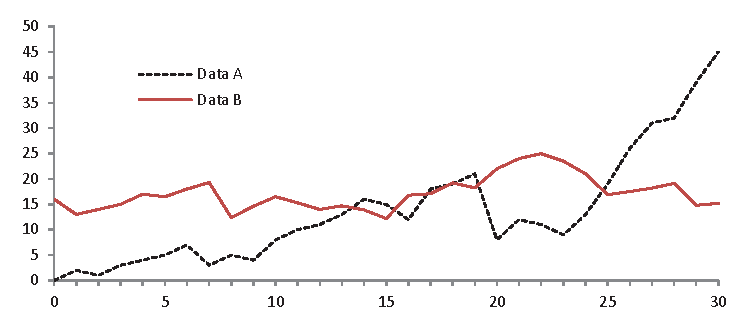
\includegraphics[width=\textwidth]{fig1.eps}
% \caption{A figure caption is always placed below the illustration.
% Please note that short captions are centered, while long ones are
% justified by the macro package automatically.} \label{fig1}
% \end{figure}

% \begin{theorem}
% This is a sample theorem. The run-in heading is set in bold, while
% the following text appears in italics. Definitions, lemmas,
% propositions, and corollaries are styled the same way.
% \end{theorem}
%
% the environments 'definition', 'lemma', 'proposition', 'corollary',
% 'remark', and 'example' are defined in the LLNCS documentclass as well.
%
% \begin{proof}
% Proofs, examples, and remarks have the initial word in italics,
% while the following text appears in normal font.
% \end{proof}
% For citations of references, we prefer the use of square brackets
% and consecutive numbers. Citations using labels or the author/year
% convention are also acceptable. The following bibliography provides
% a sample reference list with entries for journal
% articles~\cite{ref_article1}, an LNCS chapter~\cite{ref_lncs1}, a
% book~\cite{ref_book1}, proceedings without editors~\cite{ref_proc1},
% and a homepage~\cite{ref_url1}. Multiple citations are grouped
% \cite{ref_article1,ref_lncs1,ref_book1},
% \cite{ref_article1,ref_book1,ref_proc1,ref_url1}.
%
% ---- Bibliography ----
%
% BibTeX users should specify bibliography style 'splncs04'.
% References will then be sorted and formatted in the correct style.
%
% \bibliographystyle{splncs04}
% \bibliography{mybibliography}
%
\begin{thebibliography}{8}


% \bibitem{Rietveld}
% Rietveld,L. and Hoekstra,R.: YASGUI: not just another SPARQL client,
% In: The Semantic Web: ESWC 2013 Satellite Events, 78-86. Springer (2013)

% \bibitem{Yamaguchi}
% Yamaguchi,A. \textit{et~al}.:
% An intelligent SPARQL query builder for exploration of various life-science databases.
% In: The 3rd International Workshop on Intelligent Exploration of Semantic Data (IESD 2014) (2014)

\bibitem{sparql}
SPARQL 1.1 Query Language, W3C Recommendation 21 March 2013. \url{http://www.w3.org/TR/sparql11-query/}

\bibitem{rdf}
RDF 1.1 Concepts and Abstract Syntax, W3C Recommendation 25 February 2014. \url{http://www.w3.org/TR/rdf11-concepts/}

\bibitem{owl}
OWL 2 Web Ontology Language
\url{https://www.w3.org/TR/owl2-overview/}

\bibitem{spang}
Chiba, H., & Uchiyama, I. (2017). SPANG: a SPARQL client supporting generation and reuse of queries for distributed RDF databases. BMC bioinformatics, 18(1), 93.

\bibitem{umaka}
Yamamoto, Y., Yamaguchi, A., & Splendiani, A. (2018). YummyData: providing high-quality open life science data. Database, 2018.

\bibitem{fair}
Wilkinson, M. D., Dumontier, M., Aalbersberg, I. J., Appleton, G., Axton, M., Baak, A., ... & Bouwman, J. (2016). The FAIR Guiding Principles for scientific data management and stewardship. Scientific data, 3.

\bibitem{sparql-doc}
sparql-doc: Generate HTML documentation from SPARQL queries.
\url{https://github.com/ldodds/sparql-doc}

\bibitem{spin}
SPIN: SPARQL Inferencing Notation.
\url{https://spinrdf.org/}

\bibitem{rdf-portal}
Kawashima, S., Katayama, T., Hatanaka, H., Kushida, T., & Takagi, T. (2018). NBDC RDF portal: a comprehensive repository for semantic data in life sciences. Database, 2018.

\bibitem{bioportal}
Salvadores, M., Alexander, P. R., Musen, M. A., & Noy, N. F. (2013). BioPortal as a dataset of linked biomedical ontologies and terminologies in RDF. Semantic web, 4(3), 277-284.

% \bibitem{ref_article1}
% Author, F.: Article title. Journal \textbf{2}(5), 99--110 (2016)

% \bibitem{ref_lncs1}
% Author, F., Author, S.: Title of a proceedings paper. In: Editor,
% F., Editor, S. (eds.) CONFERENCE 2016, LNCS, vol. 9999, pp. 1--13.
% Springer, Heidelberg (2016). \doi{10.10007/1234567890}

% \bibitem{ref_book1}
% Author, F., Author, S., Author, T.: Book title. 2nd edn. Publisher,
% Location (1999)

% \bibitem{ref_proc1}
% Author, A.-B.: Contribution title. In: 9th International Proceedings
% on Proceedings, pp. 1--2. Publisher, Location (2010)

% \bibitem{ref_url1}
% LNCS Homepage, \url{http://www.springer.com/lncs}. Last accessed 4
% Oct 2017
\end{thebibliography}
\end{document}
